\cotefile{157-4}
\scanpage{115}
\mspage{423}
% archive sheet number: 114
% source lines 1-13
C'était là sans doute une tâche urgente. J'ai fini par comprendre pourtant qu'il y avait plus urgent encore. Il m'a fallu d'abord parer au plus pressé : renouer le contact rompu avec mon corps, l'aider à remonter de l'état d'épuisement que j'ai fini par sentir et par admettre, et à retrouver la vigueur disparue. J'ai compris alors que pour cela, il fallait que je renonce pour une durée indéterminée à toute activité intellectuelle - fut-ce celle de méditer sur le sens de ce qui m'arrivait. C'est avec les notes reprises aujourd'hui que prend fin cette longue et salutaire ``parenthèse'' dans mes grands investissements, lesquels pour un temps (\unsure{depuis} le mois de février de cette année) s'étaient rejoints dans l'écriture de ``R\,é\,c\,o\,l\,t\,e\,s\quad e\,t\quad S\,e\,m\,a\,i\,l\,l\,e\,s''. La présente note est une toute première réflexion, ou tout au moins une sorte de compte-rendu sommaire, au sujet de cette ``parenthèse'' de quatre mois.

% source lines 14-21
Le temps de comprendre, à la fin des fins, le besoin d'un repos complet, une grande fatigue était devenue un épuisement profond. Faute d'avoir su écouter le langage pourtant péremptoire de mon corps, les quelques dérisoires pages de commentaires et retouches à l'Enterrement, arrachées sur un état de fatigue physique en ces premières deux semaines, l'ont été au prix d'une mise d'énergie qui, avec le recul, me paraît démentielle ! Toujours est-il qu'après ces prouesses, il m'a fallu rester allongé pendant de longues semaines, ne me levant que quelques heures par jour pour les tâches pratiques indispensables.

% source lines 22-28
Chose remarquable, une fois c\,o\,m\,p\,r\,i\,s le besoin d'un repos complet, je n'ai pas éprouvé la moindre difficulté à décrocher complètement de toute activité intellectuelle, sans aucune velléité de ``tricher''. Je n'avais pas même à prendre de décision à proprement parler - du seul fait d'avoir compris, j'avais déjà décroché. Les tâches qui la veille encore m'avaient tenu en haleine, soudain semblaient très lointaines, comme appartenant à un passé très reculé...

% source lines 29-36
Le présent n'en était pas vide pour autant. Alors que pendant des semaines et des mois le sommeil est resté réticent à venir, et que je restais allongé de longues heures, apparemment dans l'inaction totale, je ne me rappelle pas une seule fois avoir trouvé le temps long. Je refaisais connaissance avec mon corps, et aussi avec l'environnement le plus immédiat - ma chambre, ou parfois le morceau de gazon ou d'herbes sèches baigné de soleil juste devant mes yeux, là où d'aventure je m'étais allongé, près de la maison ou au cours d'une courte (et prudente...) promenade. Je passais de longs moments à poursuivre la danse d'une
\scanpage{117}
\mspage{1}
% archive sheet number: 116
Carrés $h$-cartésiens et $h$-cocartésiens

\deleted{Structures \unsure{quadrangulées|quadrangulaires}}

1. \uline{Axiomes} de \uline{structures} \uline{\unsure{quadrangulées|quadrangulaires}} (une tentative avortée)

% source lines 1-7
Soit : $(M,W)$ une catégorie de modèles admettant une théorie de la fibre homotopique. Alors on a dans $\mathrm{Ho}_W\unsure{\mathcal C|\mathscr H|\mathcal E}=MW^{-1}$ une notion de \uline{carré} \uline{$W$-cartésien} (ou $W$-homotopiquement cartésien), par quoi on entend un diagramme carré
\diagram{\begin{tikzcd}[ampersand replacement=\&]
X_1 \arrow[d] \& X_3 \arrow[l] \arrow[d] \\
X_0 \& X_2 \arrow[l]
\end{tikzcd}}
dans $\mathrm{Ho}_W$ provenant, à iso. près, d'un carré $W$-cartésien dans $M$ - donc \deleted{\unsure{par exemple}} isomorphe, dans $\underline{\mathrm{Hom}}(\unsure{\mathbb{\Delta}|\Delta}^1\times\mathbb{\Delta}^1,\unsure{\mathrm{HO}|\mathrm{Ho}}_W)$, à un carré \deleted{\unsure{fibré}} \inserted{\uline{cartésien}}
\deleted{\unsure{les flèches}}
\diagram{\begin{tikzcd}[ampersand replacement=\&, column sep=large]
\deleted{\unsure{X_1}} \arrow[d, draw=none, "{\deleted{\unsure{\downarrow}}}" description] \& Y_1 \arrow[d,"p_1"'] \& Y_3(\simeq Y_1\times_{Y_0}Y_2) \arrow[l] \arrow[d] \\
\deleted{\unsure{X_0}} \& Y_0 \& Y_2 \arrow[l,"p_1"]
\end{tikzcd}}
, avec $p_1,p_2\in\mathrm{Fib}_W$. (En fait, il suffit de $p_1$ ou $p_2\in\mathrm{Fib}_W$ pour assurer le caractère $W$-cartésien du carré cartésien envisagé.) Je voudrais axiomatiser
% margin emphasis beside the following line
\margin{!}
cette situation, \unsure{partons|partant} \unsure{en tentant} de faire la liste des propriétés \unsure{formelles|éventuelles} essentielles de cette notion, et de la notion duale de carré $W$-cocartésien (ou $W$-homotopiquement cocartésien), dans le cas où $(M,W)$ admet une théorie de la cofibre homotopique. L'\unsure{espèce|esquisse} de structure, \unsure{serait|savoir|voire} celle des ``catégories quadrangulées'' (à gauche, à \unsure{droit|droite}, bilatères) est une variante, dans un cas
\scanpage{118}
\mspage{2}
% archive sheet number: 117
% source lines 1-9
non additif, de la notion de catégorie triangulée dégagée par Verdier. Comme celle-ci, cette notion est en fait trop faible - ce n'est \uline{pas} ``la bonne'' - mais elle a un intérêt pratique provisoire. La ``bonne'' notion (s'il en est une : \unsure{p. ex|p.-ê.} celle des dérivateurs) devrait travailler avec une notion plus fine des carrés et des carrés $W$-cartésiens, en travaillant systématiquement dans
\[
\mathrm{HO}_W(\unsure{\mathbb{\Delta}|\Delta}^1\times\mathbb{\Delta}^1)=M(\mathbb{\Delta}^1\times\mathbb{\Delta}^1)W(\mathbb{\Delta}^1\times\mathbb{\Delta}^1)^{-1}
\]
\inserted{(en \unsure{y prenant|y voyant} les ``vrais'' carrés $W$-cartésiens !)} et catégories similaires, telles que $\mathrm{HO}_W(\unsure{\Psi|\Upsilon})$, $\mathrm{HO}_W(\unsure{\Phi|\varphi})$. Mais les inclure dans une axiomatique ne \unsure{faisant} pas mention d'une Cat. de modèles $(M,W)$, revient manifestement à mettre le doigt dans l'engrenage de la notion \unsure{des|de} \unsure{dérivateurs|dérivateur}, et ce n'est pas mon propos pour l'instant.

% source lines 19-24
\uline{Définition 1} J'appelle ``\uline{catégorie à carrés $h$-cartésiens}'', ou ``\uline{catégorie quadrangulée à gauche}'', une Catégorie $\unsure{\mathscr H|\mathcal H|H}$, munie d'un sous-ensemble $\mathrm{Cart}$ de l'ens $\mathrm{Hom}_{\deleted{\unsure{\mathrm{Cat}}}}(\mathbb{\Delta}^1\times\mathbb{\Delta}^1,\mathscr H)$ des diagrammes carrés
\diagram{\begin{tikzcd}[ampersand replacement=\&]
X_1 \arrow[d] \& X_3 \arrow[l] \arrow[d] \\
X_0 \& X_2 \arrow[l]
\end{tikzcd}}
dans $\mathscr H$, carrés appelés ``\uline{$h$-cartésiens}'' ($h$ comme ``homotopiquement''), Cette
\scanpage{119}
\mspage{3}
% archive sheet number: 118 (upper left)
donnée \deleted{\unsure{est}} \inserted{étant} soumise aux axiomes qui suivent $\mathrm{Cart}(1)$ à $\mathrm{Cart}(\ldots)$.

Comme je ne suis pas sûr de connaître d'avance \inserted{toutes} les propriétés essentielles, le nombre de ces axiomes reste pour le moment ouvert.

\uline{Cart(1)} (\uline{Symétrie}) Si un carré
\diagram{\begin{tikzcd}[ampersand replacement=\&]
X_1 \arrow[d] \& X_3 \arrow[l] \arrow[d] \\
X_0 \& X_2 \arrow[l]
\end{tikzcd}}
est \inserted{$h$-}cartésien, de $=$ le carré symétrique (obtenu en échangeant le rôle de $X_1$ et de $X_2$).

\uline{Cart(2)} (\uline{Carrés triviaux}) Soit
\diagram{\begin{tikzcd}[ampersand replacement=\&]
X_1 \arrow[d,"p_1"'] \& X_3 \arrow[l,"q_2"'] \arrow[d,"q_1"] \\
X_0 \& X_2 \arrow[l,"p_2"]
\end{tikzcd}}
un carré dans $\unsure{\mathscr H|\mathcal H|H}$, avec $p_1$ un iso. Alors le carré est $h$-cartésien \unsure{sss|ssi} $q_1$ est un iso.

\uline{Cart(3)} (\uline{Carrés composés}) Soit un diagr. comm.
\diagram{\begin{tikzcd}[ampersand replacement=\&]
X'_0 \arrow[d] \arrow[dr,phantom,"{\underline{\overline{\mathrm I}}}" description] \& X'_1 \arrow[l] \arrow[d] \arrow[dr,phantom,"{\underline{\overline{\mathrm{II}}}}" description] \& X'_2 \arrow[l] \arrow[d] \\
X_0 \& X_1 \arrow[l] \& X_2 \arrow[l]
\end{tikzcd}}
, d'où les carrés $\underline{\overline{\mathrm I}}$, $\underline{\overline{\mathrm{II}}}$ et
\diagram{\begin{tikzcd}[ampersand replacement=\&]
\underline{\overline{\mathrm{III}}}: \& X'_0 \arrow[d] \& X'_2 \arrow[l] \arrow[d] \\
\& X_0 \& X_2 \arrow[l]
\end{tikzcd}}
(qu'on appelle \uline{carré composé} (``horizontal'') des carrés $\underline{\overline{\mathrm I}}$ et $\underline{\overline{\mathrm{II}}}$). Supposons $\underline{\overline{\mathrm I}}$ $h$-cartésien. Alors $\underline{\overline{\mathrm{II}}}$ est $h$-cartésien sss $\underline{\overline{\mathrm{III}}}$ l'est.

\deleted{\uline{\unsure{Cart(4)}}} \inserted{Corollaire} \deleted{(\unsure{Théorème} \unsure{des cubes})} Soit un diagramme commutatif cubique, \inserted{\unsure{qu'on}} peut considérer comme hom. d'un carré \inserted{(supérieur du cube)} dans un autre (face inférieure) :
\diagram{\begin{tikzcd}[ampersand replacement=\&,row sep=small,column sep=small]
\& {} \arrow[dl] \arrow[dd,dashed] \& \& {} \arrow[ll] \arrow[dl] \arrow[dd] \\
{} \arrow[dd] \& \& {} \arrow[ll] \arrow[dd] \& \\
\& {} \arrow[dl] \& \& {} \arrow[ll,dashed] \arrow[dl] \\
{} \& \& {} \arrow[ll] \&
\end{tikzcd}}
Toutes les faces du cube\textsuperscript{*}, \uline{sf} la face supérieure sont
% margin note written slanted, rising to the right
\margin{* En fait, il suffit de la face inférieure, et de deux faces opposées latérales (p. ex. celle de \unsure{devant} et celle de derrière)}
\scanpage{120}
\mspage{4}
% archive sheet number: 119
% margin note written slanted, rising to the right
\margin{\uline{Cor} (de $\mathrm{Cart}(3)$ et $\mathrm{Cart}(2)$) \unsure{tt} carré isomorphe à un carré $h$-cartésien est $h$-cartésien.}
des carrés $h$-cartésiens (\unsure{savoir} la face inférieure et les quatre faces latérales), il en est de même de la face supérieure.
\deleted{\uline{NB} En fait, il suffit de supposer que}

Ces axiomes sont dans la nature d'axiomes de stabilité, nous donnant des critères \unsure{suffisants} pour que certains carrés \unsure{sont|soient} $h$-cartésiens, si telles conditions sont vérifiées (p. ex. que certains autres carrés sont déjà $h$-cartésiens). J'ai l'impression d'avoir \deleted{\unsure{ici}} épuisé ici les propriétés \unsure{pertinentes} de ce type (i.e. que les autres devraient pouvoir s'en déduire). À présent, je m'occupe des propriétés d'existence et d'unicité des carrés $h$-cartésiens.

% vertical emphasis stroke beside Cart(4)
\margin{$\vert$}
\uline{Cart(\unsure{4|5})} \inserted{(Axiome des produits fibrés)} Tout diagramme
\diagram{\begin{tikzcd}[ampersand replacement=\&]
X_1 \arrow[d] \& \\
\unsure{X_0} \& X_2 \arrow[l]
\end{tikzcd}}
dans $\unsure{\mathscr H|\mathcal H|H}$ peut se \unsure{complèter|compléter} en un carré $h$-cartésien
\diagram{\begin{tikzcd}[ampersand replacement=\&]
X_1 \arrow[d] \& X_3 \arrow[l] \arrow[d] \\
X_0 \& X_2 \arrow[l]
\end{tikzcd}}
.

L'axiome suivant \inserted{(cf \unsure{son} corollaire)} \unsure{assurera|assure} que le carré $h$-cartésien en question est \inserted{\unsure{intrinsèquement}} \uline{unique à isom} près - mais on fera attention qu'il n'est en général pas unique ``à isom unique près''.

\uline{Cart(5)} \inserted{(Axiome d'exactitude)} Considérons deux \deleted{\unsure{diagr.}} carrés $h$-cartésiens
\diagram{\begin{tikzcd}[ampersand replacement=\&]
X=\Biggl( \& X_1 \arrow[d] \& X_3 \arrow[l] \arrow[d] \& \Biggr) \\
\& X_0 \& X_2 \arrow[l] \&
\end{tikzcd}}
et
\diagram{\begin{tikzcd}[ampersand replacement=\&]
Y=\Biggl( \& Y_1 \arrow[d] \& \unsure{X_3|Y_3} \arrow[l] \arrow[d] \& \Biggr) \\
\& Y_0 \& Y_2 \arrow[l] \&
\end{tikzcd}}
, et un hom. \inserted{$p=(p_0,p_1,p_2)$} entre les diagrammes de type
\diagram{\begin{tikzcd}[ampersand replacement=\&]
\unsure{\Phi|\mathscr Q}= \& 1 \arrow[d] \& \\
\& 0 \& 2 \arrow[l]
\end{tikzcd}}
associés (cf diagrammes traits pleins ci-dessous) :
\scanpage{121}
\mspage{5}
% archive sheet number: 120
\diagram{\begin{tikzcd}[ampersand replacement=\&,row sep=large,column sep=small]
\& X_{\unsure{1|4}} \arrow[dl,Rightarrow] \arrow[dd,"p_1",near start] \& \& X_3 \arrow[ll] \arrow[dl,dash] \arrow[dd,dotted,"p_3"] \\
X_0 \arrow[dd,"p_0"'] \& \& X_2 \arrow[ll] \arrow[dd,"p_2"'] \& \\
\& Y_1 \arrow[dl] \& \& Y_3 \arrow[ll] \arrow[dl] \\
Y_0 \& \& Y_2 \arrow[ll] \&
\end{tikzcd}}

Alors :

a) il existe un hom. $\bar p:X\to Y$ induisant $p$, i.e. il existe une flèche $p_3$ de façon à compléter ce diagramme cubique commutatif (en respectant donc les contraintes de commutativité pour les deux carrés adjacents à l'arête $p_3$).

b) Si de plus $p_0,p_1,p_2$ sont des iso, il en est de même de $p_3$.

Prenant le cas où $p_0,p_1,p_2$ sont des identités, on trouve :

\uline{Corollaire 1} dans les conditions de $\mathrm{Cart}(4)$, si on a \uline{deux} carrés $h$-cartésiens \inserted{$X,X'$} qui complètent
\diagram{\begin{tikzcd}[ampersand replacement=\&]
\& \& X_1 \arrow[dl] \\
\deleted{\unsure{X_0}} \& X_0 \& \\
\& \& X_2 \arrow[ul]
\end{tikzcd}}
, il existe un hom. de $\unsure{\alpha|X}$ dans $\alpha'$ qui induise l'identité sur les sommets d'indices $0,1,2$, et un tel hom. est tjrs un isomorphisme.

Mais cet isom. n'est pas forcément unique, car \unsure{d'autres|d'entrée|d'autre} \unsure{dans|de jeu|part} un autom. d'un carré \deleted{\unsure{les}} \inserted{$h$-}cartésien peut induire l'identité sur les sommets $X_0,X_1,X_2$, sans être l'identité.
\scanpage{122}
\mspage{6}
% archive sheet number: 121
\uline{Corollaire 2} Considérons un carré \deleted{$h$-cartésien}
\diagram{\begin{tikzcd}[ampersand replacement=\&,execute at end picture={
\node[anchor=east] at ([xshift=-5pt]current bounding box.west) {$\deleted{X}\unsure{Y|X}=\Biggl($};
\node[anchor=west] at ([xshift=5pt]current bounding box.east) {$\Biggr)$};
}]
\deleted{X_1}Y_1 \arrow[d] \& \deleted{X_3}Y_3 \arrow[l] \arrow[d] \\
\deleted{X_0}Y_0 \& \deleted{X_2}Y_2 \arrow[l]
\end{tikzcd}}
,
et un objet $T$ de $\unsure{\mathscr H|\mathcal H|H}$, d'où (posant $\operatorname{Hom}(T,X)=\deleted{X}Y(T)$) un carré comm. des $(\mathrm{Ens})$
\diagram{\begin{tikzcd}[ampersand replacement=\&]
\deleted{X_1}Y_1(T) \arrow[d] \& \deleted{X_3}Y_3(T) \arrow[l] \arrow[d] \\
\deleted{X_0}Y_0(T) \& \deleted{X_2}Y_2(T) \arrow[l]
\end{tikzcd}}
, et par suite
\[
\deleted{X_3}Y_3(T)\longrightarrow \deleted{X_1}Y_1(T)\mathbin{\times}_{\deleted{X_0}Y_0(T)}\deleted{X_2}Y_2(T).\tag*{(*)}
\]
Si $\deleted{X}Y$ est $h$-cartésien, cette application \inserted{$(*)$} est \uline{surjective} quel que soit $T$. \deleted{(\unsure{mais|ceci} \unsure{que}}

On applique $\operatorname{Cart}(\unsure{6|5})$ à $Y$ et au carré constant \inserted{$X$} de valeur $T$
\diagram{\begin{tikzcd}[ampersand replacement=\&,execute at end picture={
\node[anchor=east] at ([xshift=-5pt]current bounding box.west) {$X=$};
}]
T \arrow[d,"\mathrm{id}"'] \& T \arrow[l,"\mathrm{id}"'] \arrow[d,"\mathrm{id}"] \\
T \& T \arrow[l,"\mathrm{id}"]
\end{tikzcd}}
, en notant que la donnée de $p=(p_0,p_1,p_2)$ de
\diagram{\begin{tikzcd}[ampersand replacement=\&]
T \arrow[d] \& \\
T \& T \arrow[l]
\end{tikzcd}}
dans
\diagram{\begin{tikzcd}[ampersand replacement=\&]
Y_1 \arrow[d] \& \\
Y_0 \& Y_2 \arrow[l]
\end{tikzcd}}
revient à la donnée d'un élément du deuxième mb de $(*)$, et que \deleted{\unsure{l'existence d'un}}
\diagram{\begin{tikzcd}[ampersand replacement=\&]
Y_1 \arrow[d] \& T \arrow[l,"p_1"'] \arrow[d,"p_2"] \arrow[dl,dashed,"p_0"'] \\
\unsure{Y_0|\deleted{Y_0}} \& \unsure{Y_2|\deleted{Y_2}} \arrow[l]
\end{tikzcd}}
éléments \deleted{$p_3$} de $Y_3(T)$ qui s'envoient (par $*$) dans cet élément ne sont autres que les $p_3$ dont l'axiome $\operatorname{Cart}(6)$ affirme l'existence.

\uline{NB} On notera que l'application \inserted{surjective} $(*)$ n'est en général pas bijective, i.e. le carré $h$-cartésien n'est en général pas cartésien.
\scanpage{123}
\mspage{7}
% archive sheet number: 122
\uline{NB} Il y a une notion duale de \uline{catégorie à carrés $h$-cocartésiens}, ou \uline{catégorie quadrangulée à droite}. Le plus souvent, les deux structures sont présentes simultanément. Il y a lieu de dégager des propriétés qui relient les deux structures duales sur une même catégorie. \inserted{Ainsi} Sauf erreur, dans le cas \inserted{$\unsure{\mathscr H|\mathcal H|H}$} \unsure{additife|additive|additi\deleted{f}ve|additif}, les deux espèces de carrés, les $h$-cartésiens et les $h$-cocartésiens, devraient \uline{coïncider}. (\unsure{Il|Je} me faudra revenir là-dessus par la suite.) Dans le cas $\mathscr H$ ``\unsure{ponctuée|pointée}'', il y a l'adjonction des foncteurs $\Sigma,\Omega$ liés l'un à la structure quadrangulée droite, l'autre à la structure quadrangulée gauche. Et il y a, quand il y a des $\underline{\operatorname{Hom}}$ internes ou externes, des propriétés éventuelles de $\underline{\operatorname{Hom}}(X,Y)$ \unsure{p.r.|p.v.} aux quadrangles $h$-cocartésiens en $X$, $h$-cartésiens en $Y$ -- mais c'est à peine un lien entre les deux structures --

2. Exemples.

Un premier exemple trivial, est celui où $\mathscr H$ est stable par produits fibrés, et où les carrés $h$-cartésiens sont définis comme les carrés cartésiens. Les axiomes $\operatorname{Cart}(1)$ à $\operatorname{Cart}(5)$ sont des propriétés bien connues, $\pm$ tautologiques de la notion de carré cartésien. Et
\scanpage{124}
\mspage{8}
% archive sheet number: 123
en un sens, le cas général doit se ramener à ce cas particulier banal.

Le seul type \unsure{d'autres|d'autre} cas que je connaisse, est celui où $\unsure{\mathscr H|\mathcal H|H}=MW^{-1}$, où $W$ est un localiseur admettant une théorie de la fibre $W$-homotopique (cf $\underline{\overline{\mathrm{XII}}}$). Dans ce cas, on l'a dit, on prend comme carrés $h$-cartésiens dans $\mathscr H$ ceux qui sont isomorphes, dans $\underline{\operatorname{Hom}}(\unsure{\mathbb{\Delta}|\Delta}^{1}\times\mathbb{\Delta}^{1},\mathscr H)$, à un carré $W$-cartésien dans $M$. Encore faut-il vérifier les axiomes $\operatorname{Cart}(1)$ à $\operatorname{Cart}(5)$. Je pense que je n'ai guère de chance d'y arriver que moyennant une

\uline{Proposition 1}. Moyennant des hypothèses sur $(M,W)$ \unsure{pouvant|paraissant|précisant} être dégagées ci-dessous, vérifiées en tous cas où $(M,W)$ est \unsure{quarrinable|quarrable|quarrifiable} \deleted{\unsure{dég. de|degré|degré de} \unsure{uniformément|uniformité}} sur la catégorie des ens. ordonnés finis \inserted{(cf $\underline{\overline{\mathrm{XIII}}}$, p. 51)}, on a ceci :
% vertical emphasis rule alongside the proposition
\margin{$\vert$}
soit
\diagram{\begin{tikzcd}[ampersand replacement=\&,execute at end picture={\node[anchor=east] at ([xshift=-5pt]current bounding box.west) {$X=\Biggl($};\node[anchor=west] at ([xshift=5pt]current bounding box.east) {$\Biggr)$};}]
X_1 \arrow[d] \& X_3 \arrow[l] \arrow[d] \\
X_0 \& X_2 \arrow[l]
\end{tikzcd}}
un carré dans $M$, et soit $\mathrm{ho}_W(X)$ son image dans $\underline{\operatorname{Hom}}(\mathbb{\Delta}^{1}\times\mathbb{\Delta}^{1},\mathrm{Ho}_W)$.
% second vertical emphasis rule alongside the concluding lines
\margin{$\vert$}
Pour que $\mathrm{ho}_W(X)$ soit $h$-cartésien, il \uline{faut} (et il suffit, bien sûr) que $X$ soit $W$-cartésien.
\scanpage{125}
% archive sheet number: 124
$\underline{\overline{\mathrm{XV}}}$ Factorisations

Construction de Catégories de modèles et de dérivateurs (?)

Théorème principal sur $(\mathrm{Cat},\unsure{w|W})$ (p. $105$ \unsure{s.|...|i.})
\scanpage{126}
% archive sheet number: 125
Th. de factorisation principal : p. 10

Généralités sur les couples et triples de Quillen : 28-43

Ensembles \unsure{inaccessibles|accessibles} \hfill 43-73

Structures de Quillen \unsure{pour} les catégories-test ($\deleted{A}$\unsure{pour} $\widehat A,W_A$) : th. principal \hfill 105

Axiomes des localisateurs fondamentaux révisés ($\mathrm{Loc}\,1-\mathrm{Loc}\,8$) \hfill $\unsure{116|146}-\unsure{123|128|133}$ \deleted{\unsure{(suite)|120}}

\unsure{Gênes|Génér.} sur l'axiome de commut. ho. (8)
% vertical rule grouping the two preceding entries at the right
\margin{$\vert$}

Application au \unsure{bidérivateur|bifoncteur} $\unsure{\mathrm{HOT}|\mathrm{Hot}|\mathrm{HOL}}$
\scanpage{127}
\mspage{1}
% archive sheet number: 126
\uline{Théorèmes} de \uline{factorisation dans les catégories accessibles}

% slanted margin heading, read after rotation
\margin{1. \uline{Construction} \uline{fondamentale} : la suite transfinie de factorisations d'une flèche $f$}

Soit $M$ une \inserted{$\unsure{\mathcal U|U}$-}catégorie, stable par ``petites'' (i.e. $\mathcal U$-petites) $\underset{\longrightarrow}{\lim}$ filtrantes. Soit
\[C_0\subset\mathrm{Fl}\,M\tag*{1.1.}\]
un \inserted{\uline{petit}} ensemble de flèches, on se propose de construire pour toute flèche $f$ de $M$, une factorisation
\[f=pi\qquad i\in\widetilde C_0=((C_0)_*)^{\unsure{\kappa|*}},\ p\in(C_0)_*.\tag*{1.2.}\]
Pour ceci, on va construire une suite ordinale de foncteurs
\[
\left\{\begin{aligned}
f&\longmapsto\deleted{\unsure{\Sigma|Z}_\alpha}\unsure{X_\alpha|\Sigma_\alpha|Z_\alpha}(f)=\deleted{\Sigma_\alpha}X_\alpha(C_0,f)\\
\deleted{\Sigma_\alpha}X_\alpha&:\underline{\mathrm{Fl}}(M)\longrightarrow\deleted{\underline{\mathrm{Fl}}(}M\deleted{)}
\end{aligned}\right.\tag*{1.3.}
\]
\deleted{\unsure{tels que|tel que}} et des hom. fonctoriels \deleted{\unsure{avec} $f:X\longrightarrow Y$}
\deleted{$\unsure{\operatorname{source}}\,\Sigma_\alpha(f)=$}
\diagram{\begin{tikzcd}[ampersand replacement=\&]
\deleted{X} \& \deleted{\unsure{\Sigma|X|Z}_\alpha(f)} \arrow[l,"\deleted{i_\alpha(f)}"']
\end{tikzcd}}
\deleted{$\operatorname{source}f\longrightarrow X_\alpha(f)$ \unsure{l'identité} \unsure{dont}}
\[i_\alpha:\operatorname{source}f\longrightarrow X_\alpha(f)\qquad\text{(fonctoriel en $f$)}\tag*{1.4.}\]
\deleted{et un hom. fonctoriel en $f$}
\diagram{\begin{tikzcd}[ampersand replacement=\&]
\deleted{\unsure{\operatorname{but}|\operatorname{source}}}\deleted{\Sigma_\alpha}X_\alpha(f) \arrow[r,"p_\alpha(f)"] \& \operatorname{but}(f)
\end{tikzcd}}
\[\tag*{1.5.}\]
de sorte qu'on a le diagramme (où $X=\operatorname{source}f$, $Y=\operatorname{but}f$)
\diagram{\begin{tikzcd}[ampersand replacement=\&]
X \arrow[rr,dash,"f"] \arrow[dr,"\deleted{\unsure{\Sigma|I}_\alpha}i_\alpha(f)"'] \& \& Y \\
\& X_\alpha(f) \arrow[ur,"p_\alpha(f)"'] \&
\end{tikzcd}}
\[\tag*{1.6.}\]
, ce diagramme étant commutatif
\[f=p_\alpha(f)\deleted{\Sigma_\alpha}i_\alpha(f).\tag*{1.7.}\]
On peut dire aussi qu'on a une section du foncteur canonique \inserted{\unsure{dit} ``\unsure{composition}''} (transposé de $\unsure{\mathbb{\Delta}|\Delta}^{1}\longrightarrow\mathbb{\Delta}^{2}$, donné par $0\mapsto0$, $1\mapsto2$ :
\[\tag*{1.8.}\]
\diagram{\begin{tikzcd}[ampersand replacement=\&,execute at end picture={\node[anchor=east] at ([xshift=-5pt]current bounding box.west) {$\Biggl\{$};}]
\underline{\operatorname{Nerf}}_2(M) \arrow[r,"\unsure{\sigma|\rho}"] \& \underline{\operatorname{Nerf}}_1(M)=\underline{\mathrm{Fl}}(M) \arrow[l,bend left=35,dashed,"\deleted{\unsure{F}}\unsure{\Phi|\mathcal F|F}_\alpha"]
\end{tikzcd}}
, $\Phi$ comme ``factorisation''
\scanpage{128}
\mspage{2}
% archive sheet number: 127
\unsure{où}
\diagram{\begin{tikzcd}[ampersand replacement=\&,execute at end picture={
\node[anchor=east] at ([xshift=-5pt]current bounding box.west) {$\deleted{\unsure{F|P}}\unsure{\Phi|\mathcal F|F}_\alpha(f)=\Bigl\{$};
\node[anchor=west] at ([xshift=5pt]current bounding box.east) {$\Bigr\}$};}]
X \arrow[r,"\deleted{\unsure{\Sigma_\alpha|I_\alpha}}i_\alpha(f)"] \& X_\alpha(f) \arrow[r,Rightarrow,"p_\alpha(f)"] \& Y
\end{tikzcd}}
\[\tag*{1.9.}\]
avec $p_\alpha(f)\deleted{\Sigma_\alpha}i_\alpha(f)=f$. La fonctorialité de 1.4. et 1.5., ou celle de $\Phi_\alpha$ i.e. de 1.9., s'exprime par le fait que tout \deleted{diagramme}\inserted{carré} commutatif
\diagram{\begin{tikzcd}[ampersand replacement=\&]
X \arrow[r,phantom,"\unsure{\overset{f}{\longrightarrow}|\overset{f}{\longleftrightarrow}}"] \arrow[d,"u_X"'] \& Y \arrow[d,"u_Y"] \\
X' \arrow[r,"f'"'] \& Y'
\end{tikzcd}}
\[\tag*{1.10.}\]
dans $M$, interprété comme flèche $u=(u_X,u_Y)$ de $f$ dans $f'$ dans $\underline{\mathrm{Fl}}(M)$, donne \unsure{naissance} à un double carré commutatif
\diagram{\begin{tikzcd}[ampersand replacement=\&]
X \arrow[r,Rightarrow,"\deleted{\Sigma_\alpha}i_\alpha(f)"] \arrow[d,"u_X"'] \& \deleted{\unsure{\Sigma_\alpha|Z_\alpha}}X_\alpha(f) \arrow[r,"p_\alpha(f)"] \arrow[d,"X_\alpha(u)"] \& Y \arrow[d,"u_Y"] \\
X' \arrow[r,Rightarrow,"\deleted{\Sigma_\alpha}i_\alpha(f')"'] \& X_\alpha(f') \arrow[r,"p_\alpha(f')"'] \& Y'
\end{tikzcd}}
\[\tag*{1.11.}\]
.

\uline{NB} Quand on voudra expliciter la dépendance de \unsure{ces|mes} constructions p.r. à $C_0$, on écrira
% Original horizontal order retained with the handwritten transposition stroke reproduced.
\figure{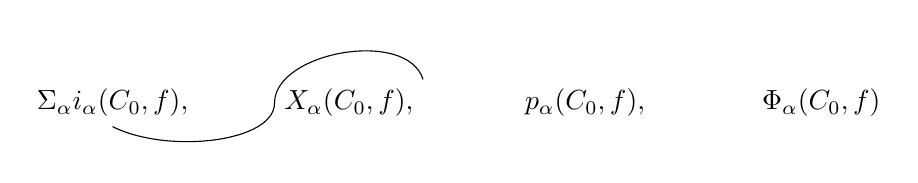
\begin{tikzpicture}
\node (a) at (0,0) {$\deleted{\Sigma_\alpha}i_\alpha(C_0,f),$};
\node (b) at (3,0) {$X_\alpha(C_0,f),$};
\node (c) at (6,0) {$p_\alpha(C_0,f),$};
\node (d) at (9,0) {$\Phi_\alpha(C_0,f)$};
\draw (a.south) .. controls +(0.7,-0.35) and +(0,-0.5) .. (b.west) .. controls +(0,0.65) and +(-0.2,0.65) .. (b.north east);
\end{tikzpicture}}
ou
\figure{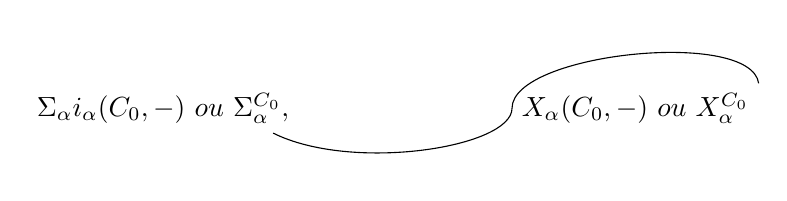
\begin{tikzpicture}
\node (a) at (0,0) {$\deleted{\Sigma_\alpha}i_\alpha(C_0,-)\ \text{ou}\ \Sigma_\alpha^{C_0},$};
\node (b) at (6,0) {$X_\alpha(C_0,-)\ \text{ou}\ X_\alpha^{C_0}$};
\draw ([xshift=1.4cm]a.south) .. controls +(1,-0.5) and +(0,-0.5) .. (b.west) .. controls +(0,0.7) and +(-0.1,0.7) .. (b.north east);
\end{tikzpicture}}
au lieu de $\deleted{\Sigma_\alpha}i_\alpha(f)\ \ldots\ ,\ \deleted{\Sigma_\alpha}i_\alpha,\ \ldots$ .

Voici les propriétés essentielles du système inductif ordinal des $\deleted{\Sigma_\alpha}X_\alpha(f)$ ou $\Phi_\alpha(f)$.
\scanpage{129}
\mspage{3}
% archive sheet number: 128
1. $\deleted{\unsure{\Sigma_0|Z_0}}X_0(f)=X$, $\deleted{\unsure{p_0|I_0|\Sigma_0}}i_0(f)=\mathrm{id}_X$, $p_0(f)=f$

(i.e. \deleted{\unsure{cette}} la factorisation $\unsure{\Phi|\mathcal F}_0(f)$ de $f$ est la factorisation triviale
\diagram{\begin{tikzcd}[ampersand replacement=\&]
X \arrow[r,"\unsure{f\mathrm d_X|\mathrm{id}_X}"] \& X \arrow[r,dash,"\deleted{\unsure{\mathrm{id}|p}}f"] \& Y
\end{tikzcd}}
)

2.
\[
\begin{aligned}
\deleted{\Sigma_\alpha}X_{\alpha+1}(f)&=X_1(p_\alpha(f))\\
i_{\alpha+1}(f)&=i_1(p_\alpha(f))\circ i_\alpha(f)\\
p_{\alpha+1}(f)&=p_1(p_\alpha(f))
\end{aligned}
\]
\diagram{\begin{tikzcd}[ampersand replacement=\&]
\begin{matrix}X\\\Vert\\\operatorname{source}f\end{matrix} \arrow[r,"i_\alpha(f)"] \arrow[rr,bend left=18,"f"] \& X_\alpha(f) \arrow[r,"p_\alpha(f)"] \arrow[dr,bend right=30,"i_1(p_\alpha(f))"'] \& \deleted{Y} \arrow[r] \arrow[r,bend left=18] \& Y \\
\& \& \begin{matrix}X_1(p_\alpha(f))\\=X_{\alpha+1}(f)\end{matrix} \arrow[ur,bend right=30] \&
\end{tikzcd}}

ou encore
\diagram{\begin{tikzcd}[ampersand replacement=\&,column sep=small]
X \arrow[rrr,"f"] \arrow[d,Rightarrow,"\mathrm{id}"] \& \& \& \deleted{Y} \arrow[r] \arrow[d,draw=none,"\deleted{\downarrow}"] \& Y \arrow[d,"\mathrm{id}"] \\
X \arrow[r,"i_\alpha(f)"] \arrow[d,Rightarrow,"\mathrm{id}"] \& X_\alpha(f) \arrow[rr,"p_\alpha(f)"] \arrow[d,Rightarrow,"\mathrm{id}"] \& \& \deleted{Y} \arrow[r] \arrow[d,draw=none,"\deleted{\downarrow}"] \& Y \arrow[d,"\mathrm{id}"] \\
X \arrow[r] \& X_\alpha(f) \arrow[r,"i_1(i_\alpha(f))"] \& \begin{matrix}X_1(p_\alpha(f))\\=X_{\alpha+1}(f)\end{matrix} \arrow[r,"p_1(p_\alpha(f))"] \& \deleted{Y} \arrow[r] \& Y
\end{tikzcd}}
\[\tag*{1.12.}\]
Le morphisme de transition $X_\alpha(f)\longrightarrow X_{\alpha+1}(f)$ est
\diagram{\begin{tikzcd}[ampersand replacement=\&]
X_\alpha(f) \arrow[r,"i_1(i_\alpha(f))"] \& X_1(p_\alpha(f))=X_{\alpha+1}(f)
\end{tikzcd}}

3. Si $\alpha$ est un ordinal limite, on a
\[
\left\{\begin{aligned}
X_\alpha(f)&=\underset{\alpha'<\alpha}{\underset{\longrightarrow}{\lim}}X_{\alpha'}(f)\\
i_\alpha(f)&=\text{morphisme canonique de }X=X_0(f)\text{ dans}\\
&\qquad\text{la limite inductive}\\
p_\alpha(f)&=\text{limite projective des }p_{\alpha'}(f):X_{\alpha'}(f)\longrightarrow Y
\end{aligned}\right.
\]
(on \unsure{peut} considérer la limite inductive \unsure{définissant} $X_\alpha(f)$ comme une limite dans ${}_{X\backslash}M_{/Y}\ \ldots$).
Les morphismes de transition
\[X_{\alpha'}(f)\longrightarrow X_\alpha(f)\qquad(\alpha'<\alpha)\]
sont les morphismes can. relatifs au syst. ind. des $X_{\alpha'}(f)$
\scanpage{130}
\mspage{4}
% archive sheet number: 129
On peut \unsure{donc|aussi} dire que la suite \deleted{transfinie}\inserted{ordinale} des factorisations fonctorielles $\unsure{\Phi|\mathcal F}_\alpha(f)$ de $f$ variable, se déduit de la factorisation \inserted{fonctorielle} $\Phi_1(f)$ de $f$
\diagram{\begin{tikzcd}[ampersand replacement=\&]
X \arrow[r,"i_1(f)"] \arrow[rr,bend left=20,"f"] \& X_1(f) \arrow[r,"p_1(f)"] \& Y
\end{tikzcd}}
par ``itération transfinie à droite'', i.e. en regardant les opérations $\Phi_\alpha$ comme des foncteurs
\[
p_\alpha\deleted{\unsure{\varphi|f}}\left\{\begin{aligned}
\underline{\mathrm{Fl}}(M)&\longrightarrow\underline{\mathrm{Fl}}(M)\\
f&\longmapsto p_\alpha(f)
\end{aligned}\right.
\]
\margin{\uline{NB} $p_\alpha$ respecte les structures de Catégorie sur $M$, via le foncteur $\operatorname{but}:\underline{\mathrm{Fl}}(M)\longrightarrow M$. i.e. $\underline{\mathrm{Fl}}(M)$ est considéré comme objet de $\mathrm{CAT}_{/M}$}
\unsure{munies|munis} de \deleted{\unsure{un foncteur}} hom. fonctoriels (au dessus de $M$)
\[\mathrm{id}_{\mathrm{Fl}\,M}\longrightarrow p_\alpha\deleted{\unsure{\Phi|\varphi}}.\]

Ainsi, si on considère
\[
\left\{\begin{aligned}
&\underline{\mathrm{Fl}}\,M\text{ comme objet de }\mathrm{CAT}_{/M}\\
&\qquad\text{par le foncteur }f\longmapsto\operatorname{but}f\\
&\text{où }\mathrm{CAT}\text{ est la catégorie des Catégories}\\
&\qquad\text{\uline{éléments de} }\unsure{\mathcal V|V|\mathcal U},\text{ univers tel que}\\
&M\in\mathcal V\text{ d'où }\left.\begin{aligned}\mathrm{Cat}^{(\unsure{\mathrm{ens}|\mathrm{et}})}&=\mathrm{Cat}^{\unsure{\mathcal U|U}}\\M,\mathrm{Fl}\,M\deleted{^{\unsure{\mathcal U|*}}}&\end{aligned}\right\}\in\mathrm{CAT}
\end{aligned}\right.
\]
on a un endofoncteur $p_1$ de $\underline{\mathrm{Fl}}(M)$ sur $M$, et un hom. fonctoriel
\[i_1:\mathrm{id}_{\underline{\mathrm{Fl}}(M)_{/M}}\longrightarrow p_1\qquad\text{i.e.}\tag*{1.13.}\]
\diagram{\begin{tikzcd}[ampersand replacement=\&]
X \arrow[rr,"f"] \arrow[dr,"i_1(f)"'] \& \& Y \\
\& \begin{matrix}X_1(f)\\\Vert\\\operatorname{source}p_1(f)\end{matrix} \arrow[ur,"p_1(f)"'] \&
\end{tikzcd}}
, et la description de la suite ordinale des endofoncteurs $p_\alpha$ de $\underline{\mathrm{Fl}}\,M_{/M}$ résulte de cette seule donnée, compte tenu que les petites limites ind. filtrées existent dans les fibres de $\underline{\mathrm{Fl}}\,M\xrightarrow{\operatorname{but}}M$, \deleted{\unsure{et}}
\scanpage{131}
\mspage{5.}
% archive sheet number: 130
\diagram{\begin{tikzcd}[ampersand replacement=\&,column sep=tiny]
X \arrow[r,"i_1(f)"] \arrow[dr,"f"'] \& X_1(f) \arrow[r,"i_1(p_1(f))"] \arrow[d,"p_1(f)"] \& X_2(f) \arrow[r] \arrow[dl,Rightarrow,"p_2(f)"] \& \cdots \& X_\alpha(f) \arrow[r,"i_1(p_\alpha(f))"] \arrow[dlll,"p_\alpha(f)"] \& X_{\alpha+1}(f) \arrow[r] \arrow[dllll,"p_{\alpha+1}(f)=p_1(p_\alpha(f))"] \& \cdots \\
\& Y \& \& \& \& \&
\end{tikzcd}}
\[\tag*{(1.14.)}\]
Donc, pour achever de définir la suite ordinale des $X_\alpha(f)$ \inserted{(munis \deleted{\unsure{de}} des $i_\alpha(f),p_\alpha(f)$)}, ou des $p_\alpha(f)$ (munis des $i_\alpha(f)$), il reste à décrire $X_1(f),i_1(f),p_1(f)$.

\deleted{\unsure{Je peux faire un}} La propriété essentielle de ce triple dont nous avons besoin est la suivante :

\deleted{Fact}

(1.15) $\operatorname{Fact}(C_0)$ (propriété de factorisation \unsure{p.r.|p.v.} à $C_0$)

Pour tout diagramme commutatif
\diagram{\begin{tikzcd}[ampersand replacement=\&,execute at end picture={
\node[anchor=east] at ([xshift=-5pt]current bounding box.west) {$D:$};}]
\deleted{X}A \arrow[r,Rightarrow,"\unsure{\xi|?|g}"] \arrow[d,"i"'] \& \deleted{B}X \arrow[d,"f"] \\
\deleted{X}B \arrow[r] \& Y
\end{tikzcd}}
avec $i\in C_0$

d'où un diagramme traits pleins
\deleted{il existe une factorisation}
\diagram{\begin{tikzcd}[ampersand replacement=\&,column sep=large]
A \arrow[r] \arrow[d,"i"'] \& \deleted{X} \arrow[r,Rightarrow] \& X \arrow[d,"i_D"] \arrow[dr,dashed,"i_1(f)"] \arrow[dd,bend right=28,dashed,"f"'] \& \\
B \arrow[rr] \& \& X_D\overset{\mathrm{def}}=\deleted{B}X\amalg_A B \arrow[r,dotted,"u_D"] \arrow[d,"p_D"] \& \deleted{\unsure{\Sigma_1|Z_1}}\unsure{X_1|X_\alpha}(f) \arrow[dl,dashed,"p_1(f)"] \\
\& \& Y \&
\end{tikzcd}}
, il existe un hom de la factorisation $f=p_Di_D$ de $f$ dans la factorisation $f=p_1(f)i_1(f)$, )
\deleted{$X$ \unsure{composé|complet}}
\deleted{i.e. une flèche dans $M_{/Y}$}

Pour \unsure{formuler} cette condition, j'ai utilisé l'existence des sommes \deleted{$\unsure{X_D|\Sigma_D|Z_D}$} \unsure{algamées|amalgamées} $\deleted{\unsure{\Sigma_D|Z_D}}X_D$, i.e. la condition \unsure{sur} $C_0$
